\usetikzlibrary{arrows.meta,shapes.multipart,patterns}

\begin{frame}{intuition: shadow stacks}
    \begin{itemize}
    \item problem with stack: easy to leak address/values because used for lots of data
    \vspace{.5cm}
    \item goal: keep sensitive data in \textbf{separate region}
        \begin{itemize}
        \item easier to kepe address secret?
        \end{itemize}
    \vspace{.5cm}
    \item can use this for (stronger?) alternative to stack canaries
    \end{itemize}
\end{frame}

\tikzset{
    stackBox/.style={very thick},
    onStack/.style={thick},
    frameOne/.style={fill=blue!15},
    frameTwo/.style={fill=red!15},
    markLine/.style={blue!50!black},
    markLineB/.style={red!90!black},
    hiLine/.style={red!90!black},
}
\begin{frame}{shadow stacks}
    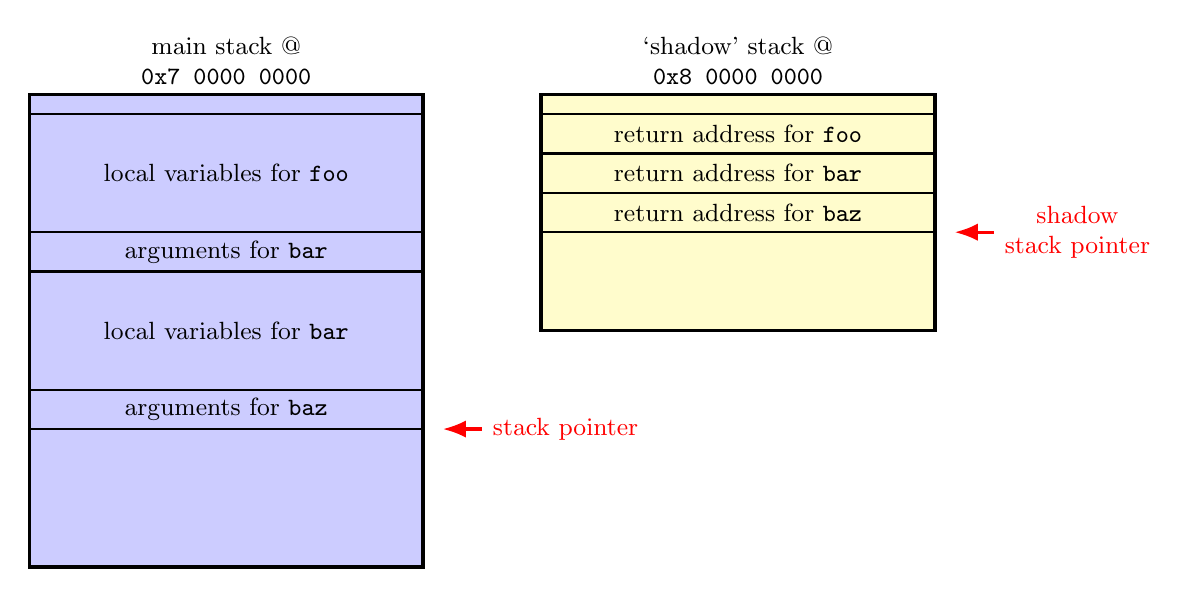
\begin{tikzpicture}
    \tikzset{
        mainSt/.style={fill=blue!20},
        otherSt/.style={fill=yellow!20},
        every node/.style={font=\small,align=center},
    }
    \draw[stackBox,mainSt] (0, 0) rectangle (5, -6);
    \node[anchor=south] at (2.5, 0) { main stack @ \\ \texttt{0x7 0000 0000}};
    \begin{scope}[yshift=-.25cm]
    \draw[onStack] (0, 0) rectangle (5, -1.5) node[midway] {local variables for \texttt{foo}};
    \draw[onStack] (0, -1.5) rectangle (5, -2) node[midway] {arguments for \texttt{bar}};
    \draw[onStack] (0, -2) rectangle (5, -3.5) node[midway] {local variables for \texttt{bar}};
    \draw[onStack] (0, -3.5) rectangle (5, -4.0) node[midway] {arguments for \texttt{baz}};
    \draw[red,very thick,Latex-] (5.25, -4.0) -- ++(.5, 0) node[right] {stack pointer};
    \end{scope}
    \node[anchor=south] at (9, 0) { `shadow' stack @ \\ \texttt{0x8 0000 0000}};
    \draw[stackBox,otherSt] (6.5, 0) rectangle (11.5, -3);
    \begin{scope}[yshift=-.25cm,xshift=6.5cm]
    \draw[onStack] (0, 0) rectangle (5, -0.5) node[midway] {return address for \texttt{foo}};
    \draw[onStack] (0, -0.5) rectangle (5, -1) node[midway] {return address for \texttt{bar}};
    \draw[onStack] (0, -1) rectangle (5, -1.5) node[midway] {return address for \texttt{baz}};
    \draw[red,very thick,Latex-] (5.25, -1.5) -- ++(.5, 0) node[right] {shadow \\stack pointer};
    \end{scope}
    \end{tikzpicture} 
\end{frame}

\begin{frame}{implementing shadow stacks}
    \begin{itemize}
    \item bigger changes to compiler than canaries
    \item more overhead to call/return from function
    \item most commonly: store return address twice
    \end{itemize}
\end{frame}

\begin{frame}[fragile,label=shadowStackx8664v1]{shadow stacks on x86-64 (1)}
\begin{itemize}
\item idea 1: dedicate \%r15 as shadow stack pointer, \\
      copy RA to shadow stack pointer in function prologue
\end{itemize}
\begin{lstlisting}[language=myasm]
function:
    movq (%rsp), %rax    // RAX <- return address
    addq $-8, %r15       // R15 <- R15 - 8
    movq %rax, (%r15)    // M[R15] <- RAX
    ...
    movq (%rsp), %rdx     // RDX <- return address
    cmpq %rdx, (%r15)    
    jne CRASH_THE_PROGRAM // if RDX != M[R15] goto CRASH_THE_PROGRAM
    add $8, %r15          // R15 <- R15 - 8
    ret
\end{lstlisting}
\end{frame}

\begin{frame}[fragile,label=shadowStackx8664v2]{shadow stacks on x86-64 (2)}
\begin{itemize}
\item idea 2: dedicate \%r15 as shadow stack pointer, \\
      avoid normal call/return instruction
\end{itemize}
\begin{lstlisting}[language=myasm]
    addq $-8, %r15
    leaq after_call(%rip), %rax
    movq %rax, (%r15)
    jmp function
after_call:

function:
    ...
    addq $8, %r15        // R15 <- R15 + 8
    jmp *-8(%r15)        // jmp M[R15-8]
\end{lstlisting}
\end{frame}

\begin{frame}[fragile,label=actShadowStack]{Android/AArch64 shadow stacks (1)}
   \begin{itemize}
    \item \tiny via \url{https://clang.llvm.org/docs/ShadowCallStack.html} (see also {\url{https://security.googleblog.com/2019/10/protecting-against-code-reuse-in-linux_30.html}})
    \item dedicate register \texttt{x18} to shadow stack pointer
        \begin{itemize}
        \item x30 = return address (after ARM's call instruction (bl))
        \end{itemize}
    \item ARM call instruction saves return address in register\ldots
    \end{itemize}
\begin{tikzpicture}
\node[draw,label={with shadow stack}] (code1) {
\begin{lstlisting}[language={},style=script]
str     x30, [x18], #8      
stp     x29, x30, [sp, #-16]!
mov     x29, sp
bl      bar
add     w0, w0, #1
ldp     x29, x30, [sp], #16
ldr     x30, [x18, #-8]!
ret
\end{lstlisting}
};
\node[anchor=north east,draw,label={without}] (code2) at (code1.north west) {
\begin{lstlisting}[language={},style=script]
stp     x29, x30, [sp, #-16]!
mov     x29, sp
bl      bar
add     w0, w0, #1
ldp     x29, x30, [sp], #16
ret
\end{lstlisting}
};
\end{tikzpicture}
\end{frame}

